\documentclass[letterpaper,12pt,titlepage, twosides, openright,abstract=on,]{report}
%letterpapper:
%12pt: tamaño de letra.
%titlepage: para crear portada.
% openright:
%abstract:

\usepackage[spanish, es-tabla]{babel}
%Este paquete pone el documento en el idioma que se le indique, en este caso es español.

\usepackage[utf8x]{inputenc} 
%Este paquete permite colocar simbolos de distintos idiomas como las tildes.

%\usepackage[document]{ragged2e}
%Este paquete permite el uso de guiones para separar palabras cuando la línea se queda demasiado corta, generado una orilla más uniforme.
%Quita la sangria!!!
\usepackage{wrapfig}
\usepackage{soul}
%Este paquete permite hacer subrayados.

\usepackage{hyperref}
%Este paquete permite crear links entre distintas partes del documento o incluso links a páginas web externas.

\usepackage{amsmath, amssymb, amsfonts}
%Estos paquetes amplían el catálogo de símbolos y entornos disponibles para escribir fórmulas matemáticas

\usepackage{graphicx}
%Este paquete permite insertar y manipular imágenes en un documento.

\usepackage{subcaption}
%Este paquete permite colocar varias imagenes.

\usepackage{blindtext}
%Este permite crear texto aleatorio.

\usepackage{siunitx}
%Este paquete permite gestionar y expresar correctamente cualquier medida utilizando el Sistema Internacional de Unidades.

\usepackage{caption}
%Este paquete permite configurar las leyendas de figuras y tablas.

\usepackage{booktabs}
%Este paquete permite añadir espacio adicional entre líneas específicas de una tabla.

\usepackage{tikz}
%Este paquete permite  generar gráficos 2D y hasta en 3D.

\usepackage{listings}
%Este paquete permite la adición de código fuente de múltiples lenguajes de programación en un documento.

\usepackage{physics}
%Este paquete permite definir macros simples y flexibles para escribir ecuaciones en los lenguajes de álgebra lineal y cálculo vectorial.

\usepackage{titlesec}
%Este paquete permite cambiar el aspecto de las unidades de estructura de un documento, como capítulos, secciones y subsecciones.

\usepackage{multirow}
%Este paquete permite construir tablas en las que algunas celdas ocupan varias filas dentro de un entorno tabular.

\usepackage[section]{placeins}
%Este paquete permite controlar la colocación de flotadores.
%section: para evitar que las figuras no procesadas correspondientes a una parte del documento se acomoden en la parte siguiente.

\usepackage{float}
%Este paquete permite rotar objetos, como tablas y figuras flotantes.
\usepackage{ragged2e}
\usepackage{xcolor}
\spanishdecimal{.}
%Este paquete cambiar el color del texto, resaltarlo de un color determinado o crear bordes a su alrededor.

\usepackage{braket}
%Este paquete permite usar la notación de bras y kets.

%\usepackage[margin=1.5cm]{geometry}

\usepackage[left=1.5cm,top=1.5cm,right=1.5cm,bottom=2cm,bindingoffset=0.5cm]{geometry}

%\setlength{\parindent}{1.27cm} %en APA se debe tener una sangria de 1.27cm
\setlength{\parskip}{2mm} %espacio entre parrafos.

\usepackage[backend=biber,style=numeric,sorting=none,autocite=inline,citestyle=apa]{biblatex}
%Este paquete permite gestionar la bibliografía de un documento.
%backend=blibtex: orden las citas
%style=numeric: Define el estilo de bibliografía y el estilo de cita
%sorting=none: Determina los criterios para ordenar las fuentes bibliográficas.
%autocite=inline:
%citestyle=phys: estilo de citación. phy: es de la APS (American Physcal Society)

\addbibresource{references.bib} %Importar el archivo .bib

%NOTA: Es indispensable colocar al final de cada capítulo el comando \newpage. Sino, no aparecera al incluirla en el comando \input{}.
%%%%%%%%%%%%%%%%%%%%%%%%%%%%%%%%%%%%%%%%%%%%
\begin{document}

\pagenumbering{roman}

\let\clearpage\relax

\hypersetup{
    colorlinks=true,
    linkcolor=black,
    citecolor=blue,
    urlcolor=blue
}
\pagenumbering{roman}

\begin{titlepage}
\centering

{\scshape\LARGE Universidad de El Salvador \par}
{\scshape\Large Facultad de Ciencias Naturales y Matemática \par}
\vspace{0.5cm}
\centering
{
\includegraphics[width=0.25\textwidth]{Chapters/1_Portada/Cover_Figures/UniversidaddeElSalvador_Logo.png}\par}
%\vspace{0.5cm}
%{\scshape\LARGE Investigación Científica \par}
\hrulefill \\
{\bfseries\LARGE{Funcionamiento un amplificador de bloqueo para su correcto uso en la solución de amplificación de señales débiles}
\par}
\hrulefill \\
\vspace{0.5cm}
{\bfseries\Large{Presentado por:} \par}
{\Large {\itshape Marlon} \par}
{\Large {\itshape Estrada} \par}
{\Large {\itshape Cindy} \par}
{\Large {\itshape Alessandra} \par}
{\Large {\itshape Eduardo 1} \par}
{\Large {\itshape Eduardo 2} \par}
{\Large {\itshape Angel} \par}
{\Large {\itshape Hellen} \par}
{\Large {\itshape ?????} \par}
{\Large {\itshape Carlos Alfredo Nuñez Cartagena} \par}
%\vfill
%{\bfseries\Large{Docente} \par}
%{\Large {\itshape Lic. Melvyn Jose Hernandez Campos} \par}
\vfill
{\Large {Ciudad Universitaria “Dr. Fabio Castillo”, 17 de octubre de 2024} \par}
\end{titlepage}

\setcounter{tocdepth}{1} %Hasta donde se desea q se vea en el indice: 0 = chapters; 1 = Sections; 2 = SubSection; 3 = Subsubsection

\tableofcontents
\addcontentsline{toc}{chapter}{\'Indice general}
\newpage

\listoffigures
\addcontentsline{toc}{chapter}{\'Indice de figuras}
\newpage

%\listoftables
%\addcontentsline{toc}{chapter}{\'Indice de tablas}
%\newpage                                       

\chapter*{Introducción} %40 por ciento
\addcontentsline{toc}{chapter}{Introducción}
%%%%%%%%%%%%%%%%%%%%%%%%%%%%%%%%%%%%%%%%%%%%%%%%%%%%%%%%%%%%%%%%
La amplificación de señales débiles es un desafío central en áreas como la física experimental, la ingeniería eléctrica y la detección de radiación. En este contexto, el amplificador de bloqueo (lock-in amplifier) es una herramienta clave para extraer señales ocultas en niveles significativos de ruido, permitiendo obtener mediciones precisas. La importancia de entender el funcionamiento de un amplificador de bloqueo radica en su capacidad para mejorar la relación señal/ruido, algo crucial en aplicaciones donde las señales son extremadamente débiles, como en la detección de partículas subatómicas, la espectroscopía y los sistemas de detección de radiación. Sin embargo, estos dispositivos presentan ciertas limitaciones, como la complejidad de su configuración y su dependencia de la frecuencia de referencia, lo que puede restringir su uso en aplicaciones que requieren respuestas rápidas o frecuencias variables.\\
\\
El objetivo de esta investigación es analizar en detalle el funcionamiento de los amplificadores de bloqueo y su correcta aplicación en la amplificación de señales débiles, explorando tanto sus ventajas como sus limitaciones técnicas. En particular, se busca comprender cómo configurar adecuadamente estos dispositivos para maximizar su efectividad, y qué factores deben considerarse para optimizar su uso en experimentos donde las señales suelen estar sumergidas en ruido. Este tema es especialmente relevante en el campo de la detección de radiación, ya que la precisión en la medición de señales débiles es un factor determinante para obtener resultados fiables.\\
\\
Este trabajo se enfocará en el estudio de un tipo específico de amplificador de bloqueo, profundizando en su funcionamiento, características y aplicaciones prácticas. Aunque existen diversas variantes de estos dispositivos, no se hará una comparación exhaustiva entre ellas, sino que se centrará en su uso básico y su optimización en condiciones experimentales. Con ello, se espera proporcionar un entendimiento claro de cómo estos amplificadores pueden ser una solución eficaz para la amplificación de señales débiles, superando los desafíos asociados a las mediciones de precisión en ambientes ruidosos.
%%%%%%%%%%%%%%%%%%%%%%%%%%%%%%%%%%%%%%%%%%%%%%%%%%%%%%%%%%%%%%%%
\newpage         
\pagenumbering{arabic}
%%%%%%%%%%%%%%%%%%%%%%%%%%%%%%%%%%%%%%%%%%%%
\chapter*{Marco Teórico} %10 por ciento
\addcontentsline{toc}{chapter}{Marco Teórico}
%%%%%%%%%%%%%%%%%%%%%%%%%%%%%%%%%%%%%%%%%%%%%%%%%%%%%%%%%%%%%%%%
Conceptos fundamentales: Definición de amplificador de bloqueo, sus componentes principales, funcionamiento básico.

Tipos de amplificadores de bloqueo: Clasificación según su aplicación, tecnología, etc. (breve)

Principios de funcionamiento: Explicación detallada de los procesos físicos involucrados en la amplificación y el bloqueo. 

Aplicaciones: Ejemplos de uso en el campo de la física de radiaciones.
%%%%%%%%%%%%%%%%%%%%%%%%%%%%%%%%%%%%%%%%%%%%%%%%%%%%%%%%%%%%%%%%
Conceptos fundamentales: Definición de amplificador de bloqueo, sus componentes principales, funcionamiento básico.

Tipos de amplificadores de bloqueo: Clasificación según su aplicación, tecnología, etc. (breve) 

Principios de funcionamiento: Explicación detallada de los procesos físicos involucrados en la amplificación y el bloqueo. 

Aplicaciones: Ejemplos de uso en el campo de la física de radiaciones.
%%%%%%%%%%%%%%%%%%%%%%%%%%%%%%%%%%%%%%%%%%%%%%%%%%%%%%%%%%%%%%%%
\section*{Desarrollo del problema}
\addcontentsline{toc}{section}{Desarrollo del problema} %Eduardo

\subsection*{xxx}
\addcontentsline{toc}{subsection}{xxx}

\subsection*{Detectores de radiación semiconductores}
\addcontentsline{toc}{subsection}{Detectores de radiación semiconductores}
%%%%%%%%%%%%%%%%%%%%%%%%%%%%%%%%%%%%%%%%%%%%%%%%%%%%%%%%%%%%%%%%
\section*{Desarrollo del problema}
\addcontentsline{toc}{section}{Desarrollo del problema} %Eduardo

\subsection*{xxx}
\addcontentsline{toc}{subsection}{xxx}
%%%%%%%%%%%%%%%%%%%%%%%%%%%%%%%%%%%%%%%%%%%%
\newpage        
\chapter*{Metodología Experimental} %15 por ciento
\addcontentsline{toc}{chapter}{Metodología Experimental}
La investigación se llevará a cabo mediante un diseño de revisión bibliográfica, complementado con simulaciones que permitan entender y analizar el funcionamiento de los amplificadores de bloqueo en la amplificación de señales débiles. Este enfoque permitirá reunir información teórica y práctica sobre el tema, facilitando un análisis más profundo. La selección de fuentes incluirá una variedad de materiales relevantes, tales como libros especializados, artículos científicos revisados por pares, patentes y bases de datos académicas. Estas fuentes se elegirán por su calidad, relevancia y actualidad, asegurando que la información recopilada sea sólida y pertinente para el estudio.\\
\\
La recolección de datos se realizará a partir de la información obtenida de las simulaciones. Estas simulaciones se diseñarán para replicar diferentes escenarios en los que se utilizan amplificadores de bloqueo, permitiendo observar su comportamiento bajo diversas condiciones y ajustando los parámetros necesarios para maximizar la amplificación de señales débiles.\\
\\
Finalmente, se llevará a cabo un análisis de datos utilizando técnicas estadísticas y cualitativas. Se emplearán métodos estadísticos para evaluar la efectividad de las configuraciones de los amplificadores de bloqueo, así como análisis cualitativos para interpretar los resultados de las simulaciones y la información obtenida de la revisión bibliográfica. Este enfoque integrador permitirá extraer conclusiones significativas sobre el funcionamiento y la optimización de los amplificadores de bloqueo en la detección de señales débiles.
%%%%%%%%%%%%%%%%%%%%%%%%%%%%%%%%%%%%%%%%%%%%%%%%%%%%%%%%%%%%%%%%
\section*{Desarrollo del problema}
\addcontentsline{toc}{section}{Desarrollo del problema} %Eduardo

El problema central de este proyecto es la necesidad de amplificar señales extremadamente débiles, que suelen estar sumergidas en ruido de fondo, un reto común en la detección de radiación y en otras áreas de la física experimental. La amplificación de estas señales es crucial para obtener mediciones precisas y confiables, pero lograrlo presenta desafíos significativos. Los amplificadores de bloqueo han sido una solución eficaz para extraer señales débiles en condiciones ruidosas, sin embargo, su correcta configuración y operación es compleja. La dependencia de la frecuencia de referencia y la sensibilidad al ruido limitan su efectividad en situaciones donde las señales fluctúan o son dinámicas, lo que plantea la necesidad de una optimización cuidadosa de sus parámetros operativos.\\
\\
Se plantea como hipótesis que una configuración optimizada del amplificador de bloqueo, ajustando adecuadamente los parámetros de frecuencia y sensibilidad al ruido, permitirá una amplificación eficiente de señales débiles, minimizando las limitaciones técnicas asociadas. Además, se espera que la mejora en la configuración maximice el rendimiento del amplificador en la detección de señales débiles en presencia de ruido.\\
\\
Para resolver este problema, es necesario responder varias preguntas: ¿Qué configuraciones y ajustes permiten una amplificación óptima de señales débiles utilizando un amplificador de bloqueo?, ¿Cuáles son los principales factores que limitan el rendimiento de estos dispositivos en la detección de señales?, ¿Qué tipos de señales se benefician más del uso de amplificadores de bloqueo y cómo se pueden adaptar los parámetros para trabajar eficazmente con diferentes niveles de ruido de fondo?.




\subsection*{Desarrollo experimental}
\addcontentsline{toc}{subsection}{Desarrollo experimental}

Dado que esta investigación se basa en una revisión bibliográfica, se utilizará el simulador LIA Simulation para ayudar a interpretar el funcionamiento de los amplificadores de bloqueo y proporcionar una comprensión más profunda de su operación en la amplificación de señales débiles. Este enfoque permitirá abordar las hipótesis planteadas y responder las preguntas de investigación de manera efectiva, para lo cual se realizaran 3 etapas; una prueba previa en el cual se familiarizara la interfaz y configuración del simulador, una serie de simulaciones en las cuales se estudiara los efectos del amplificador y como ultima etapa una posprueba para poner a prueba los conocimientos aprendidos en las 2 etapas anteriores. 

\subsubsection{Prueba Previa}
Para el análisis del simulador, es necesario conocer los siguientes símbolos, mostrados en la Tabla \ref{tab:3}.

\begin{table}[h]
\centering
\resizebox{\columnwidth}{!}{%
\begin{tabular}{cccc}
\toprule
Símbolos & Significado  \\
\midrule
$f_S$ & Frecuencia de la señal de entrada\\
$f_R$ & Frecuencia de la referencia de bloqueo \\
$f_C$ & Frecuencia de la señal de entrada sinusoidal adicional (o ruido coherente) \\
$f_{AM}$ & Frecuencia de la modulación de amplitud de la señal de entrada\\
$A_S$ & Amplitud de la señal de entrada\\
$A_C$ & Amplitud de la señal de entrada sinusoidal adicional (o ruido coherente)\\
$P_{AM}$ & Porcentaje de amplitud agregado a la amplitud como modulación de amplitud\\
$\eta$ & Definido aquí (Aumentar este valor aumenta la intensidad de este ruido)\\
$\phi$ & Ángulo de fase de la señal de entrada con respecto a la señal de referencia\\
$\tau$ & Constante de tiempo (el “ms” que aparece en esta simulación significa milisegundos) \\
$V_{MX}$ & Salida del amplificador lock-in en fase con la referencia antes del filtro de paso bajo\\
$V_{MY}$ & Salida del amplificador lock-in desfasada con la referencia antes del filtro de paso bajo\\
$V_{OutX}$ & Salida del amplificador lock-in en fase con la referencia\\
$V_{OutY}$ & Salida del amplificador lock-in desfasada con respecto a la referencia\\
\bottomrule
\end{tabular}%
}
\caption{Variables utilizadas en el simulador}
\label{tab:3}
\end{table}

Ahora podemos realizar las siguientes demostraciones del simulador.

\begin{table}[H]
\centering
\resizebox{0.55\columnwidth}{!}{ % Ajusta el tamaño al 90% del ancho de la columna
\begin{tabular}{c|c|c} % Definir columnas
    \hline
    \textbf{Variable} & \textbf{Valor} & \textbf{Resultados} \\
    \hline
    $f_s$   & 80 & \multirow{6}{*}{%
    \begin{minipage}{.25\textwidth}
    \centering
    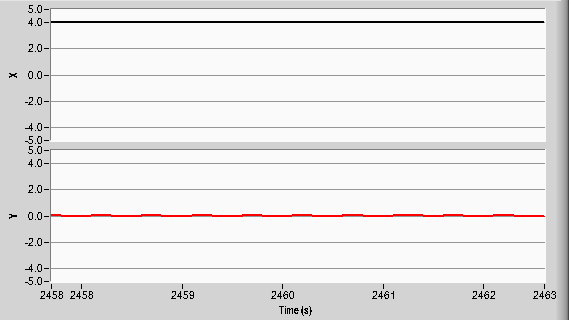
\includegraphics[width=1.2\textwidth]{Chapters/4_Metodología/Imagenes/1.png} \\
    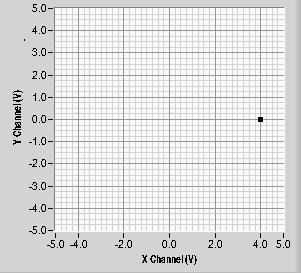
\includegraphics[width=1.2\textwidth]{Chapters/4_Metodología/Imagenes/2.png}
    \end{minipage}} \\
    $f_R$ & 80 \\
    $f_C$ & 60 \\
    $f_{AM}$ & 0\\
    $A_S$ & 4\\
    $A_C$ & 1\\
    $P_{AM}$ & 0\\
    $\eta$ & 0\\
    $\phi$ & 0\\
    $\tau$ & 1 \\
    $V_{MX}$ & 4\\
    $V_{MY}$ & 1\\
    $V_{OutX}$ & 4\\
    $V_{OutY}$ & 0\\
    Entrada sinusoidal & desactivada\\
    Filtro de paso bajo & activado \\
    \hline
\end{tabular}
}
\caption{Variables utilizadas en el simulador con sus respectivas salidas.}
\end{table}

\begin{table}[H]
\centering
\resizebox{0.55\columnwidth}{!}{ % Ajusta el tamaño al 90% del ancho de la columna
\begin{tabular}{c|c|c} % Definir columnas
    \hline
    \textbf{Variable} & \textbf{Valor} & \textbf{Resultados} \\
    \hline
    $f_s$   & 100 & \multirow{6}{*}{%
    \begin{minipage}{.25\textwidth}
    \centering
    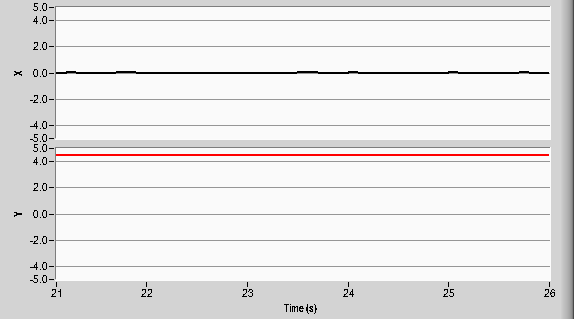
\includegraphics[width=1.2\textwidth]{Chapters/4_Metodología/Imagenes/3.png} \\
    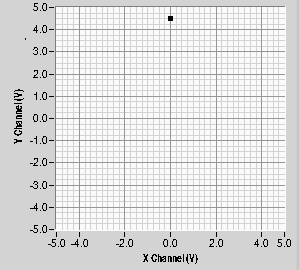
\includegraphics[width=1.2\textwidth]{Chapters/4_Metodología/Imagenes/4.png}
    \end{minipage}} \\
    $f_R$ & 100 \\
    $f_C$ & 60 \\
    $f_{AM}$ & 0\\
    $A_S$ & 4.5\\
    $A_C$ & 1\\
    $P_{AM}$ & 0\\
    $\eta$ & 0\\
    $\phi$ & 90\\
    $\tau$ & 1 \\
    $V_{MX}$ & 4.5\\
    $V_{MY}$ & 1\\
    $V_{OutX}$ & 0\\
    $V_{OutY}$ & 4.5\\
    Entrada sinusoidal & desactivada\\
    Filtro de paso bajo & activado \\
    \hline
\end{tabular}
}
\caption{Variables utilizadas en el simulador con sus respectivas salidas.}
\end{table}

\begin{table}[H]
\centering
\resizebox{0.55\columnwidth}{!}{ % Ajusta el tamaño al 90% del ancho de la columna
\begin{tabular}{c|c|c} % Definir columnas
    \hline
    \textbf{Variable} & \textbf{Valor} & \textbf{Resultados} \\
    \hline
    $f_s$   & 250 & \multirow{6}{*}{%
    \begin{minipage}{.25\textwidth}
    \centering
    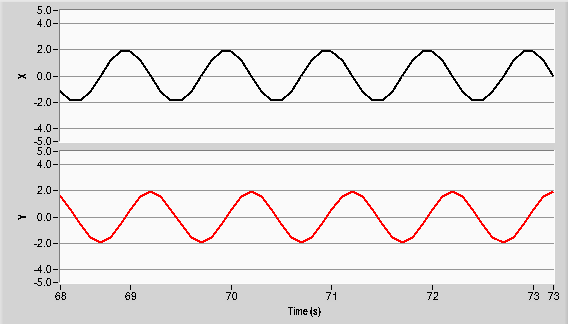
\includegraphics[width=1.2\textwidth]{Chapters/4_Metodología/Imagenes/5.png} \\
    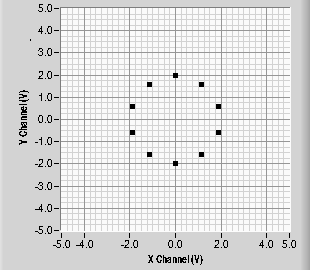
\includegraphics[width=1.2\textwidth]{Chapters/4_Metodología/Imagenes/6.png}
    \end{minipage}} \\
    $f_R$ & 249 \\
    $f_C$ & 60 \\
    $f_{AM}$ & 0\\
    $A_S$ & 2\\
    $A_C$ & 1\\
    $P_{AM}$ & 0\\
    $\eta$ & 0\\
    $\phi$ & 0\\
    $\tau$ & 25m \\
    $V_{MX}$ & 2\\
    $V_{MY}$ & 1\\
    $V_{OutX}$ & 2\\
    $V_{OutY}$ & 2\\
    Entrada sinusoidal & desactivada\\
    Filtro de paso bajo & activado \\
    \hline
\end{tabular}
}
\caption{Variables utilizadas en el simulador con sus respectivas salidas.}
\end{table}


\begin{table}[H]
\centering
\resizebox{0.55\columnwidth}{!}{ % Ajusta el tamaño al 90% del ancho de la columna
\begin{tabular}{c|c|c} % Definir columnas
    \hline
    \textbf{Variable} & \textbf{Valor} & \textbf{Resultados} \\
    \hline
    $f_s$   & 260 & \multirow{6}{*}{%
    \begin{minipage}{.25\textwidth}
    \centering
    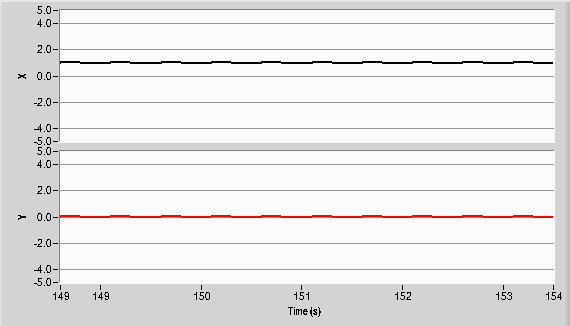
\includegraphics[width=1.2\textwidth]{Chapters/4_Metodología/Imagenes/7.png} \\
    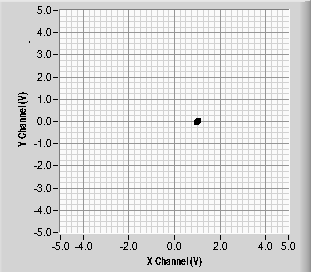
\includegraphics[width=1.2\textwidth]{Chapters/4_Metodología/Imagenes/8.png}
    \end{minipage}} \\
    $f_R$ & 260 \\
    $f_C$ & 2\\
    $f_{AM}$ & 0\\
    $A_S$ & 1\\
    $A_C$ & 3\\
    $P_{AM}$ & 0\\
    $\eta$ & 0\\
    $\phi$ & 0\\
    $\tau$ & 50m \\
    $V_{MX}$ & 4\\
    $V_{MY}$ & 1\\
    $V_{OutX}$ & 1\\
    $V_{OutY}$ & 0\\
    Entrada sinusoidal & activado\\
    Filtro de paso bajo & activado \\
    \hline
\end{tabular}
}
\caption{Variables utilizadas en el simulador con sus respectivas salidas.}
\end{table}

\begin{table}[H]
\centering
\resizebox{0.55\columnwidth}{!}{ % Ajusta el tamaño al 90% del ancho de la columna
\begin{tabular}{c|c|c} % Definir columnas
    \hline
    \textbf{Variable} & \textbf{Valor} & \textbf{Resultados} \\
    \hline
    $f_s$   & 250 & \multirow{6}{*}{%
    \begin{minipage}{.25\textwidth}
    \centering
    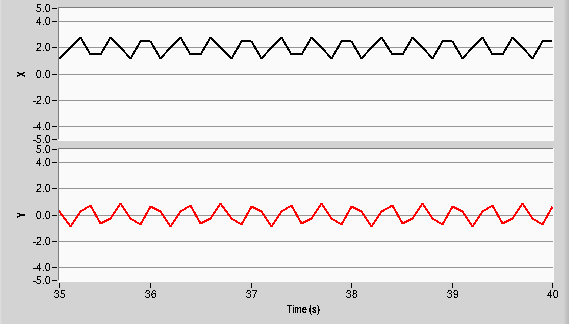
\includegraphics[width=1.2\textwidth]{Chapters/4_Metodología/Imagenes/9.png} \\
    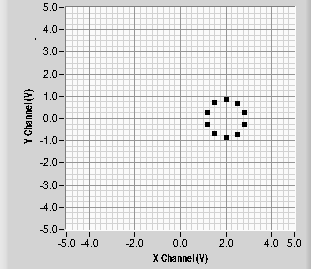
\includegraphics[width=1.2\textwidth]{Chapters/4_Metodología/Imagenes/10.png}
    \end{minipage}} \\
    $f_R$ & 250 \\
    $f_C$ & 253\\
    $f_{AM}$ & 0\\
    $A_S$ & 2\\
    $A_C$ & 1\\
    $P_{AM}$ & 0\\
    $\eta$ & 0\\
    $\phi$ & 0\\
    $\tau$ & 20m \\
    $V_{MX}$ & 3\\
    $V_{MY}$ & 1\\
    $V_{OutX}$ & 3\\
    $V_{OutY}$ & 1\\
    Entrada sinusoidal & activado\\
    Filtro de paso bajo & activado \\
    \hline
\end{tabular}
}
\caption{Variables utilizadas en el simulador con sus respectivas salidas.}
\end{table}


\begin{table}[H]
\centering
\resizebox{0.55\columnwidth}{!}{ % Ajusta el tamaño al 90% del ancho de la columna
\begin{tabular}{c|c|c} % Definir columnas
    \hline
    \textbf{Variable} & \textbf{Valor} & \textbf{Resultados} \\
    \hline
    $f_s$   & 120 & \multirow{6}{*}{%
    \begin{minipage}{.25\textwidth}
    \centering
    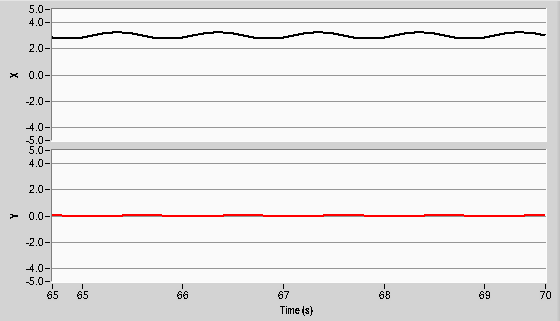
\includegraphics[width=1.2\textwidth]{Chapters/4_Metodología/Imagenes/11.png} \\
    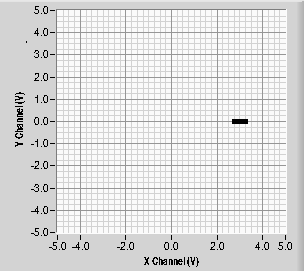
\includegraphics[width=1.2\textwidth]{Chapters/4_Metodología/Imagenes/12.png}
    \end{minipage}} \\
    $f_R$ & 120 \\
    $f_C$ & 253\\
    $f_{AM}$ & 0\\
    $A_S$ & 3\\
    $A_C$ & 1\\
    $P_{AM}$ & 50\\
    $\eta$ & 0\\
    $\phi$ & 0\\
    $\tau$ & 15 \\
    $V_{MX}$ & (4,-4)\\
    $V_{MY}$ & (1,-1)\\
    $V_{OutX}$ & (2.5,3.5)\\
    $V_{OutY}$ & 0\\
    Entrada sinusoidal & desactivado\\
    Filtro de paso bajo & activado \\
    \hline
\end{tabular}
}
\caption{Variables utilizadas en el simulador con sus respectivas salidas.}
\end{table}


Con esto podremos completar los parámetros necesarios para producir las siguientes señales:


\begin{table}[H]
\centering
\resizebox{0.55\columnwidth}{!}{ % Ajusta el tamaño al 90% del ancho de la columna
\begin{tabular}{c|c|c} % Definir columnas
    \hline
    \textbf{Variable} & \textbf{Valor} & \textbf{Resultados} \\
    \hline
    $f_s$   &  & \multirow{6}{*}{%
    \begin{minipage}{.25\textwidth}
    \centering
    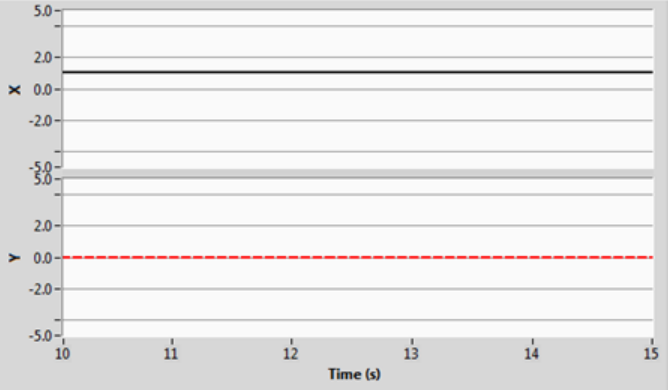
\includegraphics[width=1.2\textwidth]{Chapters/4_Metodología/Imagenes/13.png} \\
    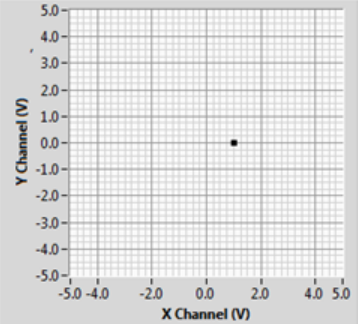
\includegraphics[width=1.2\textwidth]{Chapters/4_Metodología/Imagenes/14.png}
    \end{minipage}} \\
    $f_R$ & 20 \\
    $f_C$ & \\
    $f_{AM}$ & 0\\
    $A_S$ & \\
    $A_C$ & \\
    $P_{AM}$ & 0\\
    $\eta$ & 0\\
    $\phi$ & 0\\
    $\tau$ & 500m \\
    $V_{MX}$ & \\
    $V_{MY}$ & \\
    $V_{OutX}$ & 1\\
    $V_{OutY}$ & 0\\
    Entrada sinusoidal & opcional\\
    Filtro de paso bajo & activado \\
    \hline
\end{tabular}
}
\caption{Primera configuración a resolver utilizando el Simulador LIA.}
\end{table}


\begin{table}[H]
\centering
\resizebox{0.55\columnwidth}{!}{ % Ajusta el tamaño al 90% del ancho de la columna
\begin{tabular}{c|c|c} % Definir columnas
    \hline
    \textbf{Variable} & \textbf{Valor} & \textbf{Resultados} \\
    \hline
    $f_s$   &  & \multirow{6}{*}{%
    \begin{minipage}{.25\textwidth}
    \centering
    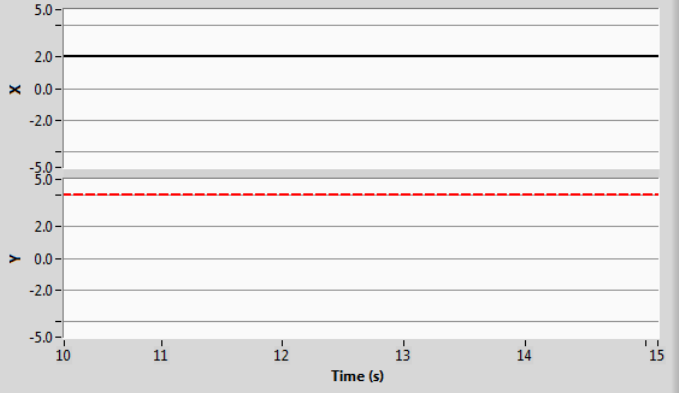
\includegraphics[width=1.2\textwidth]{Chapters/4_Metodología/Imagenes/15.png} \\
    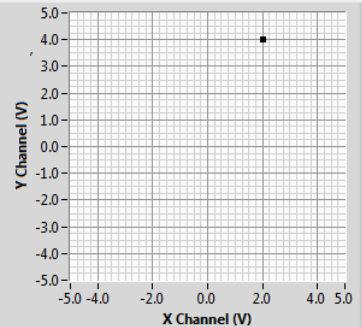
\includegraphics[width=1.2\textwidth]{Chapters/4_Metodología/Imagenes/16.png}
    \end{minipage}} \\
    $f_R$ & 35 \\
    $f_C$ & \\
    $f_{AM}$ & 0\\
    $A_S$ & \\
    $A_C$ & \\
    $P_{AM}$ & 0\\
    $\eta$ & 0\\
    $\phi$ & 0\\
    $\tau$ & 3 \\
    $V_{MX}$ & \\
    $V_{MY}$ & \\
    $V_{OutX}$ & 2\\
    $V_{OutY}$ & 4\\
    Entrada sinusoidal & opcional\\
    Filtro de paso bajo & activado \\
    \hline
\end{tabular}
}
\caption{Segunda configuración a resolver utilizando el Simulador LIA.}
\end{table}


\begin{table}[H]
\centering
\resizebox{0.55\columnwidth}{!}{ % Ajusta el tamaño al 90% del ancho de la columna
\begin{tabular}{c|c|c} % Definir columnas
    \hline
    \textbf{Variable} & \textbf{Valor} & \textbf{Resultados} \\
    \hline
    $f_s$   &  & \multirow{6}{*}{%
    \begin{minipage}{.25\textwidth}
    \centering
    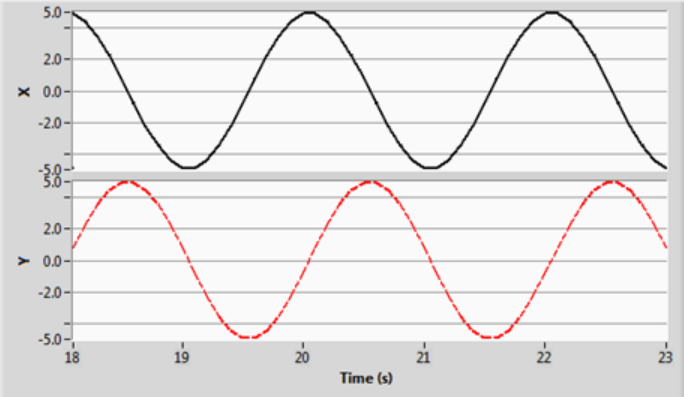
\includegraphics[width=1.2\textwidth]{Chapters/4_Metodología/Imagenes/17.png} \\
    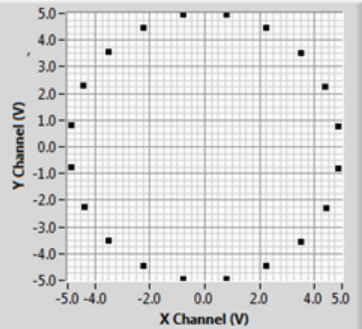
\includegraphics[width=1.2\textwidth]{Chapters/4_Metodología/Imagenes/18.png}
    \end{minipage}} \\
    $f_R$ & 50 \\
    $f_C$ & \\
    $f_{AM}$ & 0\\
    $A_S$ & \\
    $A_C$ & \\
    $P_{AM}$ & 0\\
    $\eta$ & 0\\
    $\phi$ & 0\\
    $\tau$ & 500m \\
    $V_{MX}$ & \\
    $V_{MY}$ & \\
    $V_{OutX}$ & (5,-5)\\
    $V_{OutY}$ & (5,-5)\\
    Entrada sinusoidal & opcional\\
    Filtro de paso bajo & activado \\
    \hline
\end{tabular}
}
\caption{Tercera configuración a resolver utilizando el Simulador LIA.}
\end{table}


\begin{table}[H]
\centering
\resizebox{0.55\columnwidth}{!}{ % Ajusta el tamaño al 90% del ancho de la columna
\begin{tabular}{c|c|c} % Definir columnas
    \hline
    \textbf{Variable} & \textbf{Valor} & \textbf{Resultados} \\
    \hline
    $f_s$   &  & \multirow{6}{*}{%
    \begin{minipage}{.25\textwidth}
    \centering
    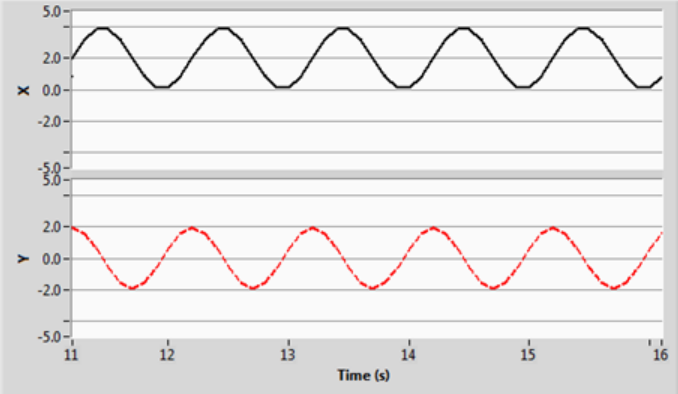
\includegraphics[width=1.2\textwidth]{Chapters/4_Metodología/Imagenes/19.png} \\
    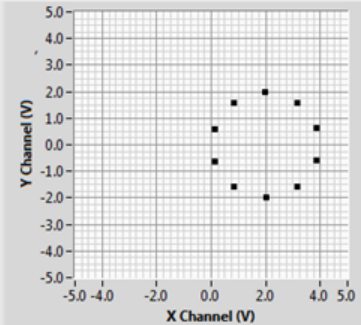
\includegraphics[width=1.2\textwidth]{Chapters/4_Metodología/Imagenes/20.png}
    \end{minipage}} \\
    $f_R$ & 0.50 \\
    $f_C$ & \\
    $f_{AM}$ & 0\\
    $A_S$ & \\
    $A_C$ & \\
    $P_{AM}$ & 0\\
    $\eta$ & 0\\
    $\phi$ & 0\\
    $\tau$ & 20m \\
    $V_{MX}$ & \\
    $V_{MY}$ & \\
    $V_{OutX}$ & (0,4)\\
    $V_{OutY}$ & (2,-2)\\
    Entrada sinusoidal & opcional\\
    Filtro de paso bajo & activado \\
    \hline
\end{tabular}
}
\caption{Cuarta configuración a resolver utilizando el Simulador LIA.}
\end{table}


Continuando con las etapas de medición con el simulador, se muestran las simulaciones ejecutas en esta etapa:


\begin{table}[H]
\centering
\resizebox{0.55\columnwidth}{!}{ % Ajusta el tamaño al 90% del ancho de la columna
\begin{tabular}{c|c|c} % Definir columnas
    \hline
    \textbf{Variable} & \textbf{Valor} & \textbf{Resultados} \\
    \hline
    $f_s$   & 10 & \multirow{6}{*}{%
    \begin{minipage}{.25\textwidth}
    \centering
    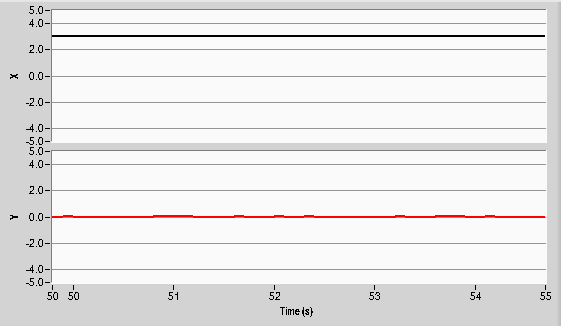
\includegraphics[width=1.3\textwidth]{Chapters/4_Metodología/Imagenes/1s.png} \\
    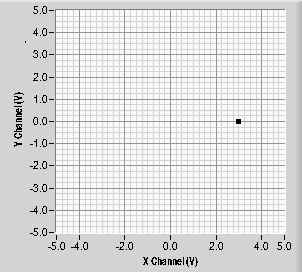
\includegraphics[width=1.3\textwidth]{Chapters/4_Metodología/Imagenes/2s.png}
    \end{minipage}} \\
    $f_R$ & 10 \\
    $f_C$ & 60\\
    $f_{AM}$ & 0\\
    $A_S$ & 3\\
    $A_C$ & 1\\
    $P_{AM}$ & 0\\
    $\eta$ & 0\\
    $\phi$ & 0\\
    $\tau$ & 2 \\
    $V_{MX}$ & (3,-3)\\
    $V_{MY}$ & (1,-1)\\
    $V_{OutX}$ & 3\\
    $V_{OutY}$ & 0\\
    Entrada sinusoidal & desactivado\\
    Filtro de paso bajo & activado \\
    Seguimiento automático & desactivado\\
    \hline
\end{tabular}
}
\caption{Simulación 1: Demostrando uno de los usos más comunes del amplificador lock-in. Medir la amplitud de una frecuencia específica en la señal de entrada configurando $f_S=f_R$.
}
\end{table}





%%%%%%%%%%%%%%%%%%%%%%%%%%%%%%%%%%%%%%%%%%%%%%%%%%%%%%%%%%%%%%%%
\newpage
            
\chapter*{Resultados  y discusión}
\addcontentsline{toc}{chapter}{Resultados y discusión}
%%%%%%%%%%%%%%%%%%%%%%%%%%%%%%%%%%%%%%%%%%%%%%%%%%%%%%%%%%%%%%%%
\blindtext
%%%%%%%%%%%%%%%%%%%%%%%%%%%%%%%%%%%%%%%%%%%%%%%%%%%%%%%%%%%%%%%%
\section*{Desarrollo del problema} %10 por ciento
\addcontentsline{toc}{section}{Desarrollo del problema} 

Presentación del problema: Descripción detallada del problema central que se abordará en el proyecto. 

Hipótesis: ¿Cuáles son las posibles soluciones o explicaciones al problema? 

Preguntas de investigación: ¿Qué preguntas específicas deben responderse para resolver el problema?

\subsection*{xxx}
\addcontentsline{toc}{subsection}{xxx}

\subsection*{Detectores de radiación semiconductores}
\addcontentsline{toc}{subsection}{Detectores de radiación semiconductores}
%%%%%%%%%%%%%%%%%%%%%%%%%%%%%%%%%%%%%%%%%%%%%%%%%%%%%%%%%%%%%%%%
\section*{Desarrollo de la solución (desarrollo experimental} %10 por ciento
\addcontentsline{toc}{section}{Desarrollo de la solución (desarrollo experimental}

Como se trata de una investigación bibliográfica, se usara un simulador de amplificador de bloqueo para ayudar a interpretar mejor el funcionamiento

Investigación individual y grupal: Búsqueda de información relevante, discusión de ideas, análisis de diferentes enfoques. 

Diseño del uso de un simulador virtual para sustituir la experimentación simulaciones: Si es necesario, diseño experimental en una simulación que ayude a la obtención de datos y facilite el entendimiento del funcionamiento del amplificador de bloqueo

Análisis de resultados: Interpretación de los datos obtenidos y comparación con las hipótesis iniciales.

\subsection*{xxx}
\addcontentsline{toc}{subsection}{xxx}
%%%%%%%%%%%%%%%%%%%%%%%%%%%%%%%%%%%%%%%%%%%%
\newpage             
\chapter*{Conclusiones y recomendaciones}
\addcontentsline{toc}{chapter}{Conclusiones y recomendaciones}

Resumen de los hallazgos: Síntesis de los resultados más importantes.

Respuesta a las preguntas de investigación: ¿Se lograron los objetivos planteados?

Limitaciones del estudio: ¿Qué aspectos no se pudieron abordar? 

Implicaciones: ¿Qué consecuencias tienen los resultados obtenidos para el campo de estudio y para futuras investigaciones?

\paragraph{Conclusiones:}
\blindtext
%%%%%%%%%%%%%%%%%%%%%%%%%%%%%%%%%%%%%%%%%%%%%%%%%%%%%%%
\paragraph{Recomendaciones:}
\blindtext
%%%%%%%%%%%%%%%%%%%%%%%%%%%%%%%%%%%%%%%%%%%%%%%%%%%%%%%
\newpage         
\chapter*{Referencias bibliográficas}
\addcontentsline{toc}{chapter}{Referencias bibliográficas}

\printbibliography[heading=none]

\newpage
%%%%%%%%%%%%%%%%%%%%%%%%%%%%%%%%%%%%%%%%%%%%
\end{document}